% This is LLNCS.DEM the demonstration file of
% the LaTeX macro package from Springer-Verlag
% for Lecture Notes in Computer Science,
% version 2.3 for LaTeX2e
%
\documentclass{llncs}
%
\usepackage{ngerman}
\usepackage[T1]{fontenc}
\usepackage[utf8]{inputenc}
\usepackage{makeidx}  % allows for indexgeneration
\usepackage{multirow}
\usepackage{rotating}
\usepackage{verbatim}
\usepackage{graphicx}
\usepackage{amssymb}   % AMS-Sonderzeichen
\usepackage{tabularx}  % Für tabularx und newcolumntype
\usepackage[paper=a4paper,left=25mm,right=25mm,top=25mm,bottom=25mm]{geometry}
\usepackage{array}
\usepackage{makecell}
\usepackage{color}
\usepackage{ragged2e}
\usepackage{ifpdf}
% \usepackage{titlesec}
\usepackage{xcolor}    % Lieber xcolor als color. Dann klappt auch das listings gut mit den Farben
\usepackage{listings}
\usepackage{upquote}   % Verändert die Ausgabe der einfachen Anführungszeichen innerhalb von verbatim
\usepackage{eurosym}   % Euro-Zeichen: \euro
\usepackage{lastpage}  % \pageref{LastPage} um die Anzahl der Seiten zu erhalten
% hiermit kann man auch umlaute copy-pasten
\usepackage{lmodern}
\selectlanguage{english}
\usepackage{fancyhdr}
\usepackage{url}
\usepackage{caption}
\captionsetup[table]{skip=10pt} % Adjust the value of '10pt' as needed
\pagestyle{fancy}


%

\ifpdf
\pdfinfo{
   /Author (Wladymir Alexander Brborich Herrera)
   /Author (Vishwaben Pareshbhai Kakadiya)
   /Author (Hellyben Bhaveshkumar Shah)
   /Author (Heer Rakeshkumar Vankawala)
   /Author (Priyanka Dilipbhai Vadiwala)
   /Title  (LowTech GMmBH Techincal Transformation Milestone 1)
   /Subject (Cloud Computing)
   /Keywords (Cloud Computing, Technical Transformation, Migration)
}
\fi

\setlength{\parindent}{0pt}    % Erste Zeile eines Absatzes nicht einrücken
\parskip2ex                    % Absatzabstand
\setlength{\itemsep}{0ex plus0.2ex}
\sloppy                        % Auf jeden Fall die Seitenränder einhalten.

\newcommand{\what}{LowTech GMmBH Techincal Transformation Milestone 1}
\newcommand{\who}{Group 23}
\newcommand{\when}{WiSe 2024-2025}

\renewcommand{\headrulewidth}{0.4pt}
\renewcommand{\footrulewidth}{0.4pt}
\lhead[\when]{\who}
\rhead[\who]{\when}
\chead[]{}
\lfoot[Page \thepage\ of \pageref{LastPage}]{\what}
\rfoot[\what]{Page \thepage\ of \pageref{LastPage}}
\cfoot[]{}
\pagestyle{fancy}


% Hurenkinder und Schusterjungen komplett verbieten.
\clubpenalty = 10000 
\widowpenalty = 10000 
\displaywidowpenalty = 10000
% Diese Begriffe bezeichnen den Makel beim Textsatz, wenn eine Seite mit der ersten Zeile eines Absatzes endet (so genannter Schusterjunge) oder eine neue Seite mit der letzten Zeile eines Absatzes beginnt (so genanntes Hurenkind).


% Wir definieren ein paar Farben
\definecolor{Brown}{cmyk}{0,0.81,1,0.60}
\definecolor{OliveGreen}{cmyk}{0.64,0,0.95,0.40}
\definecolor{CadetBlue}{cmyk}{0.62,0.57,0.23,0}
\definecolor{lightlightgray}{gray}{0.9}
\definecolor{FrankfurtBlue}{HTML}{3333b2}

% Hier fängt das Dokument an!
\begin{document}

%
% \frontmatter          % for the preliminaries
%
% \tableofcontents
%
\mainmatter              % start of the contributions
%
\title{\what}
%
\author{
  Wladymir Alexander Brborich Herrera\\
  \texttt{wladymir.brborich-herrera@stud.fra-uas.de}
  \and\\ 
  Vishwaben Pareshbhai Kakadiya\\
  \texttt{vishwaben.kakadiya@stud.fra-uas.de}
  \and\\
  Hellyben Bhaveshkumar Shah (1476905)\\
  \texttt{hellyben.shah@stud.fra-uas.de}
  \and\\
  Heer Rakeshkumar Vankawala (1449039
  )\\
  \texttt{heer.vankawala@stud.fra-uas.de}
  \and\\S
  Priyanka Dilipbhai Vadiwala\\
  \texttt{priyanka.vadiwala@stud.fra-uas.de}
}
%
\institute{
  Frankfurt University of Applied Sciences\\
  (1971-2014: Fachhochschule Frankfurt am Main)\\
  Nibelungenplatz 1\\
  D-60318 Frankfurt am Main\\
}

\maketitle              % typeset the title of the contribution

\begin{abstract}
  In this report, we as consultants from \textit{Awesome Cloud AG} present a technical transformation analysis aimed at modernizing the infrastructure of \textit{LowTech GmbH}, 
  a small to medium-sized enterprise specializing in wooden furniture production. 
  The analysis includes a critical assessment of the current infrastructure, energy consumption calculation for the existing setup 
  followed by a detailed transformation roadmap of future-ready modern infrastructure and explanations of enhancements in scalability, availability, and security compared to current infrastructure. 
  This analysis will serve as a foundational step for subsequent project phases, ensuring that \textit{LowTech GmbH} is well-equipped to meet future requirements and challenges.
\end{abstract}

This is where the introduction (the prologue or foreword) comes in. The introduction should also be short and concise. The reader should be prepared for the text that follows. Of course, the introduction should also be formulated in an interesting way.

\section{Overview of the problem}

LowTech GmbH has seven departments with all of their infrastructure hosted on premise. The original partner in charge of the infrastructure has gone out of business


\section{Objectives of the technological transformation}

The main high level objective is to migrate the current infrastructure into a private-cloud context, meaning that we are going to rent server space and manage only the software components of the technology stack. The hardware maintenance and provisioning will be handled by a third party. We expect to have an improvement in performance just by the fact that we will be using newer/faster technologies, nevertheless, we expect at least parity with the current implementation. 

\section{Assessment of the current (as-is) infrastructure}

\subsection{Current traffic and usage}

\subsection{Scalability, Availability and Security Analysis}
According to NIST definition of cloud computing is given as ``Cloud computing is a model for enabling ubiquitous, convenient, on-demand network access to a shared
pool of configurable computing resources (e.g., networks, servers, storage, applications, and services) that
can be rapidly provisioned and released with minimal management effort or service provider interaction.'' \cite{mell2011nist}

As \textit{LowTech GmbH} is based on Legacy IT infrastructure and currently lacking \textit{NIST five
  essential characteristics} such as On-demand self-service, Broad network access,Resource pooling,Rapid elasticity and Measured service.

\subsubsection*{Elasticity / Scalability}

\begin{itemize}
  \item \textbf{Fixed Hardware \& Inflexible Infrastructure}:
        \\
        Current infrastructure consists of 7 on-premises servers housed in a single 19-inch rack, 
        along with 17 clients and 19 laptops all with predetermined, static configurations. 
        Moreover, the physical constraints of the on-premises setup, with no additional space for expansion, severely limit scaling options. 
        This inflexibility makes it challenging to accommodate growth or adapt to changing business needs.
        \\
  \item \textbf{Absence of Resource Utilization/pooling}:
        \\ 
        There's no apparent way to quickly scale resources up or down based on demand or user traffic fluctuation in the current infrastructure. 
        Each application typically runs on a dedicated server with fixed resources. 
        This approach leads to inefficient resource utilization, as some servers may be underutilized while others are overloaded which may lead to performance issues during peak times or resource waste during low-demand periods due to no dynamic resource allocation.
        \\
  \item \textbf{Manual Processes \& High Cost}:
        \\ 
        Any changes in capacity would likely require manual hardware upgrades or replacements including hardware installation,
        and configuration, making the process time-consuming and potentially leading to downtime.
        Replacement of hardware is not only tedious but also financially burdensome due to high costs of new hardware.
        
\end{itemize}

\subsubsection*{Availability}
\begin{itemize}
  \item \textbf{Obsolate Hardware/OS \& Runtime Environments}:
        \\
        Many components of the current infrastructure is based on very old hardware and outdated operating systems such as 
        Windows XP SP3 (Finance clients), Windows 7 SP3 (HR clients and Customer Service laptops), Debian 5.0 Lenny (Warehouse clients and server),
        Ubuntu 16.04 LTS (Sales CRM Storage server) etc. Several applications are running on outdated software versions such as Java 1.7/1.8, 
        MySQL 5.5/5.7, PHP 5.3 and Firefox 3.6 etc. which makes this whole infrastructure more susceptible to failure.
        \\
  \item \textbf{Lack of Redundancy and Backup Mechanism}:
        \\ 
        There's no mention of redundant systems or data backup solutions which might lead to significant service disruptions as well as data loss in case of any system failure.
        \\
  \item \textbf{Manual Maintainance}:
        \\It is impossible to meet high availability requirements without a robust failover mechanism due to manual maintenance operations. 
        This increases the possiblity of human errors, leads to longer downtime and reduces overall reliability.
        \\
\end{itemize}

\subsubsection*{Security}
\begin{itemize}
  \item \textbf{Basic Windows Firewall and pSense}:
        \\
        Many components of the current infrastructure is based on very old hardware and outdated operating systems such as 
        Windows XP SP3 (Finance clients), Windows 7 SP3 (HR clients and Customer Service laptops), Debian 5.0 Lenny (Warehouse clients and server),
        Ubuntu 16.04 LTS (Sales CRM Storage server) etc. Several applications are running on outdated software versions such as Java 1.7/1.8, 
        MySQL 5.5/5.7, PHP 5.3 and Firefox 3.6 etc. which makes this whole infrastructure more susceptible to failure.
        \\
  \item \textbf{Lack of Redundancy and Backup Mechanism}:
        \\ 
        There's no mention of redundant systems or data backup solutions which might lead to significant service disruptions as well as data loss in case of any system failure.
        \\
  \item \textbf{Manual Maintainance}:
        \\It is impossible to meet high availability requirements without a robust failover mechanism due to manual maintenance operations. 
        This increases the possiblity of human errors, leads to longer downtime and reduces overall reliability.
        \\
\end{itemize}
\subsection{Energy consumption and approximate cost}

Energy consumption calculation for the as-in infrastructure of Low Tech GmbH is as follows : 

\begin{table}[htbp]
  \centering
  \begin{tabular}{|l|c|c|c|c|c|}
    \hline
    \textbf{Departments} & \textbf{Server}          & \textbf{Client}          & \textbf{Laptop}          & \textbf{Total Power}   & \textbf{Annual Energy}      \\
                         & \textbf{ (Qty x Power) } & \textbf{ (Qty x Power) } & \textbf{ (Qty x Power) } & \textbf{ Consumption } & \textbf{ Consumption(KWh) } \\
    \hline
    Finance              & 1 x 1000W                & 4 x 500W                 & -                        & 3000W                  & 26,280                      \\
    \hline
    HR                   & 1 x 1000W                & 3 x 500W                 & -                        & 2500W                  & 21,900                      \\
    \hline
    Warehouse            & 1 x 1000W                & 10 x 500W                & -                        & 6000W                  & 52,560                      \\
    \hline
    Sales                & \makecell{1 x 1000W                                                                                                                   \\ 1 x 1200W} & - & 10 x 50W & 2700W & 23,652 \\
    \hline
    Operations           & 1 x 1200W                & -                        & 4 x 50W                  & 1400W                  & 12,264                      \\
    \hline
    Customer Service     & -                        & -                        & 5 x 100W                 & 500W                   & 4,380                       \\
    \hline
    Webshop              & 1 x 1200W                & -                        & -                        & 1200W                  & 10,512                      \\
    \hline
  \end{tabular}
  \caption{Power Consumption by Department and Device Type}
  \label{tab:power_consumption}
\end{table}

\textbf{Total Energy Consumption (Annual)} : 151,548 KWh (151.548 MWh)

According to Eurostat published data of electricity prices for non-household consumers \cite{eurostat2023}, Low Tech GmbH falls under the annual energy consumption band 
`IB (20 MWh to 499 MWh)' with energy price 0.3244 \EUR{} per KWh.


\textbf{Total Cost for Energy Consumption (Annual)} : 151,548 KWh x 0.3244 \EUR{} = 49,162.17 \EUR{}

\section{Client Requirements}

\begin{itemize}
  \item Make the infrastructure more scalable, available and secure
  \item Modernize the technology, runtime and operation modality
  \item Perform the migration with a maximum downtime of 4 hours
  \item Cost reduction
  \item Maintenance reduction
  \item High availability of 99.5\%
\end{itemize}

\section{Assessment of potential technological components}

\subsection{Hardware}

\begin{itemize}
  \item Provisioning modern hardware locally
  \item Renting server space
\end{itemize}

\subsection{Virtualization technologies}


\subsection{Application components}

\subsection{Platforms}

\subsection{Security components}


\section{Migration to a private-cloud context}

To perform a successful migration to a private cloud context we have analyzed the baseline performance of the current system, as well as the technologies used. Based on the client requirements, we have selected technologies and established a roadmap to perform this task.   

\subsection{Selected technologies}

\begin{itemize}
  \item Virtualization engine
  \item Storage arrangement
  \item 
\end{itemize}

\newpage

\subsection{Architecture}

\begin{figure}[htbp]
  \begin{center}
    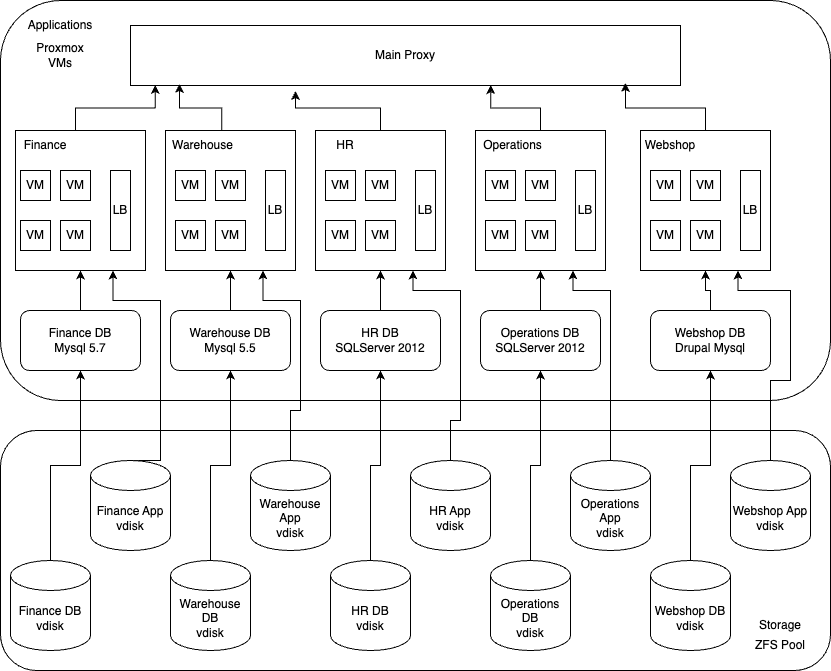
\includegraphics[width=11cm]{diagrams/architecture.drawio.png}
    \caption{High Level Architecture~\ref{High_Level_Architecture}}
    \label{High_Level_Architecture} % A unique label.
  \end{center}
\end{figure}

Note: We could use one VM and Docker to run most of the database instances as containers, making it easier to install or upgrade versions. Nevertheless, some of the tools are difficult to dockerize (SQLServer 2012) and, we want to have isolation between departments, preventing a single point of failure for all our database infrastructure.

\begin{figure}[htbp]
  \begin{center}
    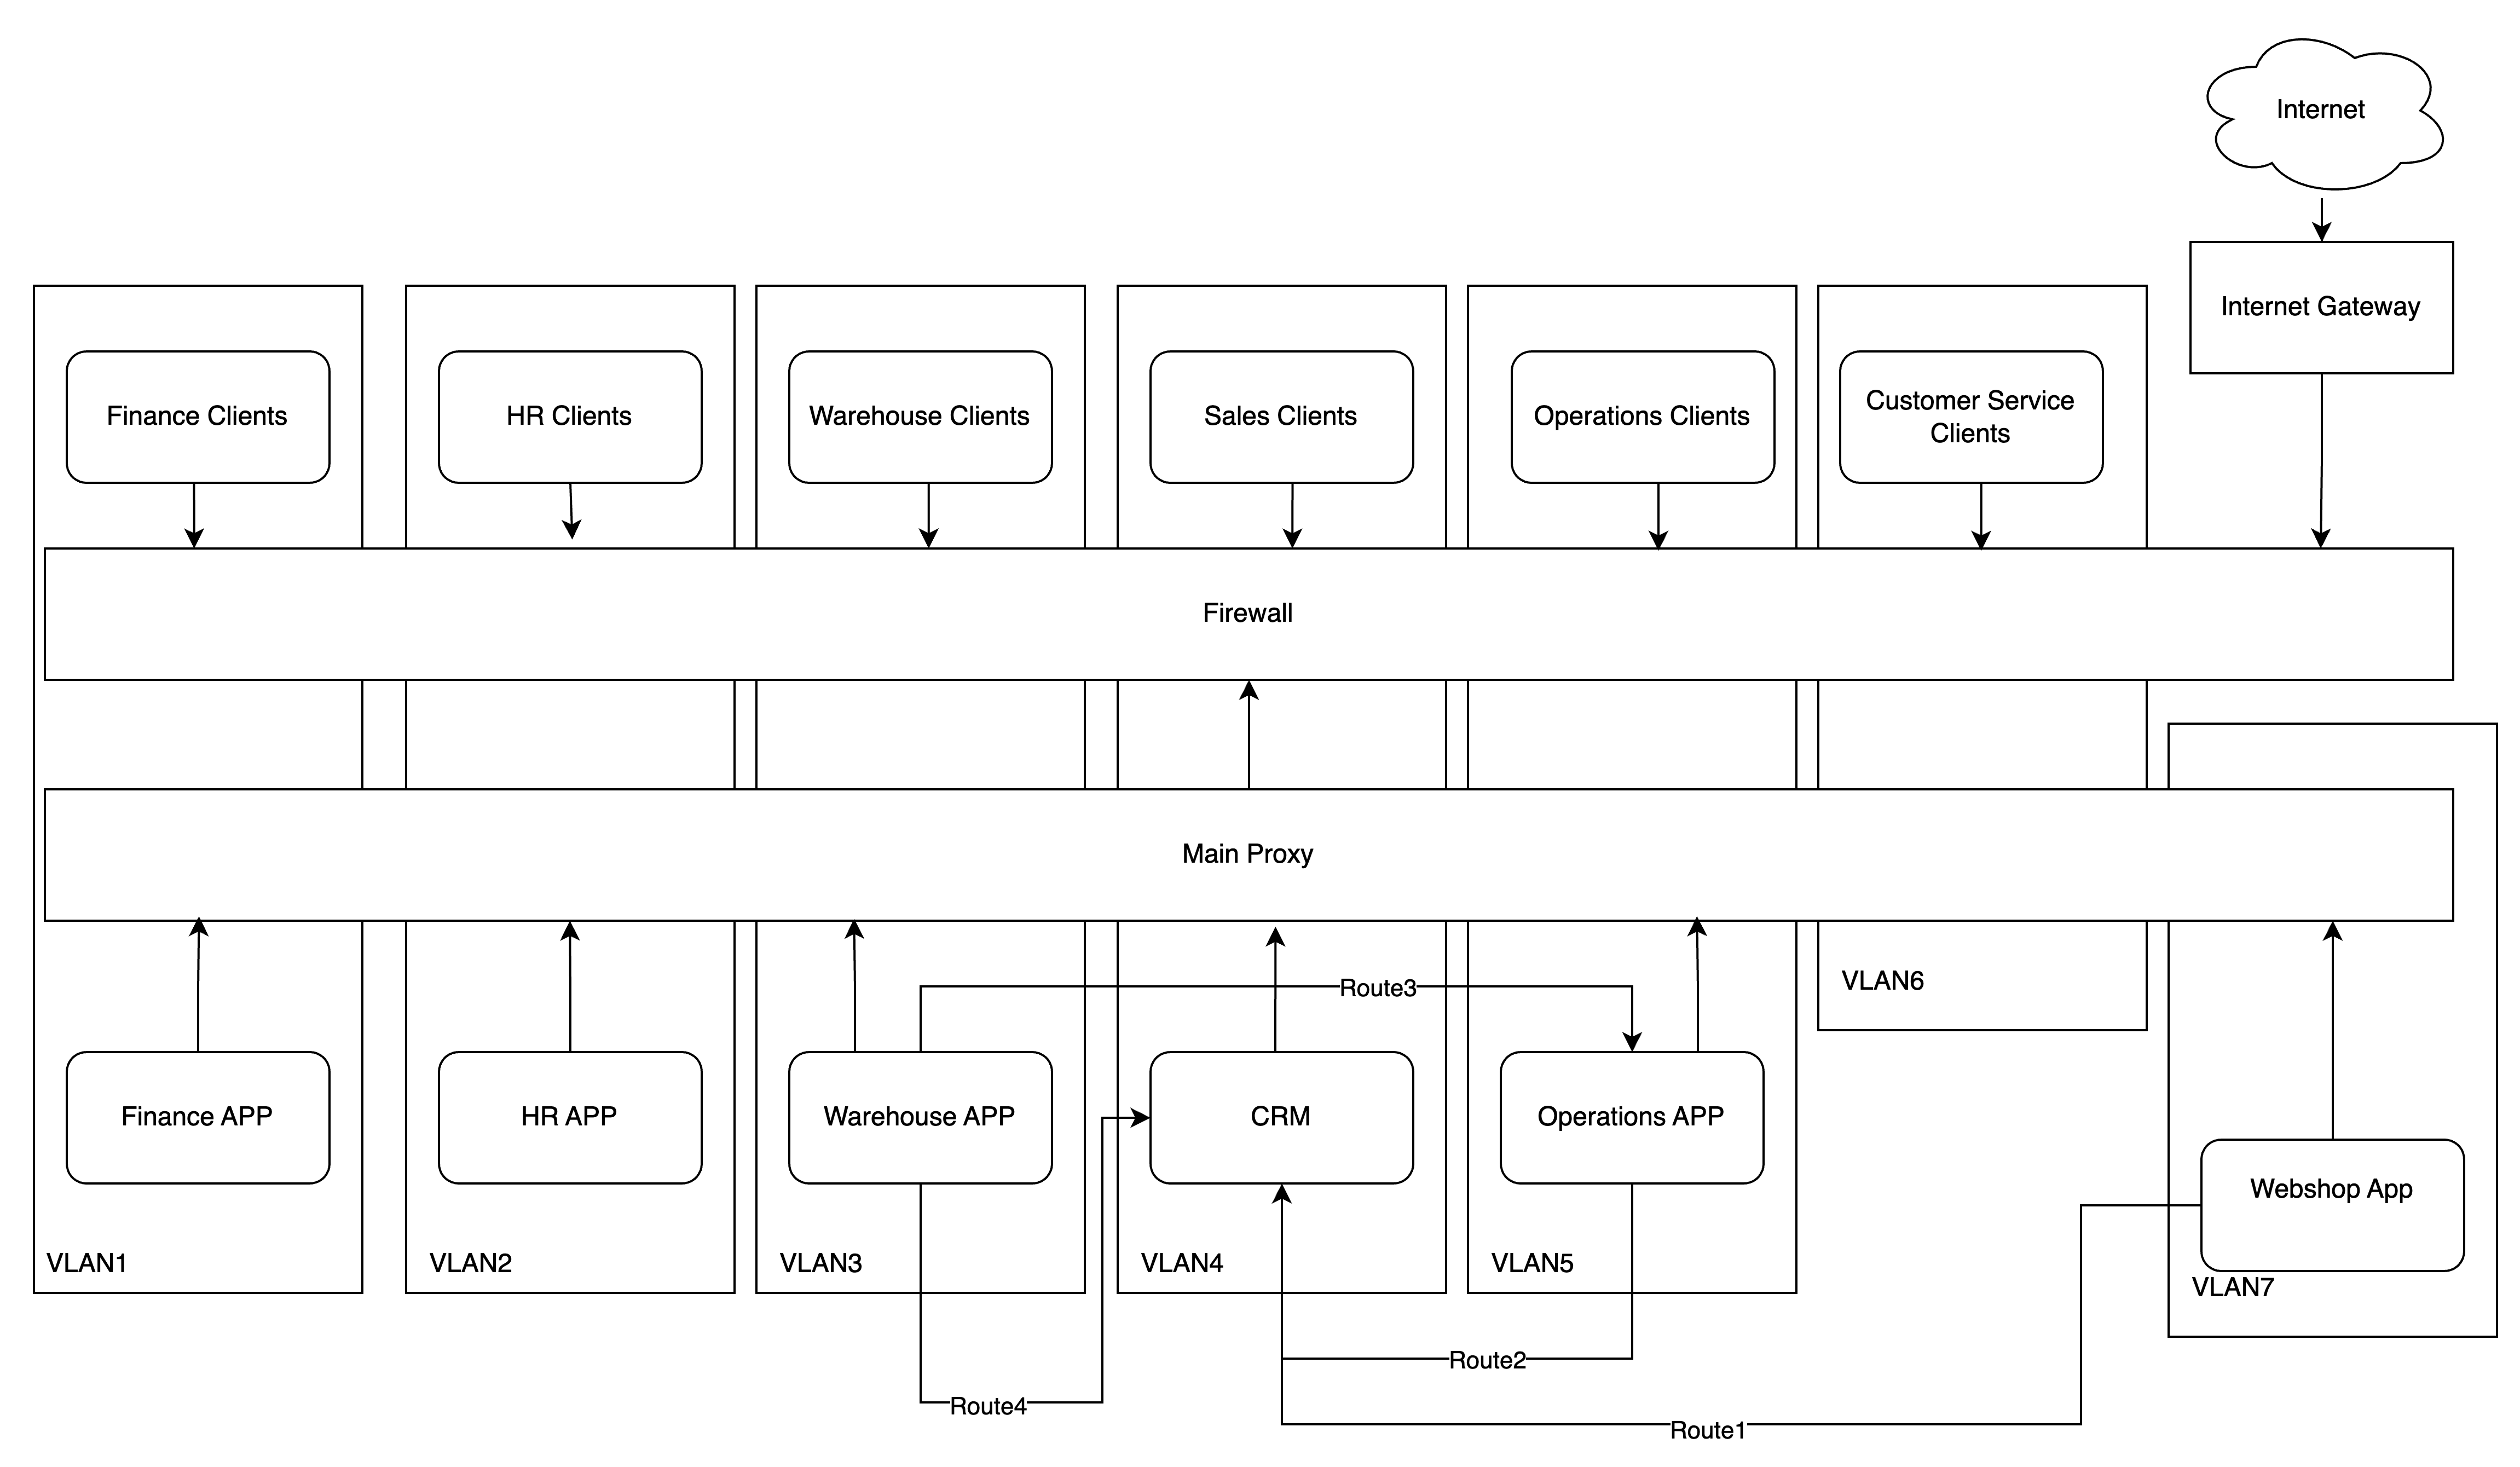
\includegraphics[width=11cm]{diagrams/network_architecture.png}
    \caption{Network Architecture~\ref{Network_Architecture}}
    \label{Network_Architecture} % A unique label.
  \end{center}
\end{figure}

We subdivide each department into its own network, virtually limiting the access of different clients to their corresponding systems. And only systems can have cross department routes to stablish communication for normal operation. 

\section{Roadmap}

The technological transformation roadmap is divided in four phases: Assessment, Design, Execution, and Optimization.

\subsection{Assessment}
This is the most critical step. We need to establish a baseline of performance, and cost of the current infrastructure. During this stage we are going to execute the following tasks:

\begin{itemize}

  \item Review the current infrastructure in terms of performance, data requirements, availability and security. Establishing baseline metrics we then have some rough idea of the areas we want to pay attention, and  at the end, the total impact that the migration had. We have some rough figures provided by the client, but these are not enough to actually guide development.
  \item Check the current applications, to define a migration approach, if they can be migrated, changed, or improved in a way that makes the transition process easier. Given the initial requirements, we can assume that the applications are not actively being developed, so modernization is not an approach we can consider at that level.
  \item Identify the level of effort per department/application/domain to make the migration, this metrics will guide the order of the execution. This is to reduce the impact of the migration in the business operation. Naturally there will be usage patterns more friendly to upgrade and intervention.
  \item Assess the budget and space constraints for new hardware, or to rent such services. A preliminary review points to renting server space as the most appropriate solution. To achieve the availability metrics required by the customer will require a great investment in provisioning, modernizing and validating the current server location. Not only in technological terms, but also: physical security, thermal management, internet bandwidth and energy provisioning.
  \item Spec the hardware after evaluating the usage pattern and metrics. We want to, not only get parity to the current hardware but have space to grow.
\end{itemize}

\subsection{Design}

In this step we perform the following tasks:

\begin{itemize}

  \item Design the new architecture diagram with networking isolation between domains, dividing each department appropriately.
  \item Document which applications will be migrated to new technologies, or will be ported as is.
  \item Create document with detailing the dates and approximate duration of the migration each application. This is to be distributed to the organization so operation disruption is minimized
  \item Prepare contingency plans, and fallbacks to minimize disruption to the business if a migration fails. This could take the form of rollbacks, traffic duplication or A/B testing. Depending on the need of each department and the complexity of each application
  \item Create all the technical documentation regarding the implementation for the application migrations to new technologies.
\end{itemize}

\subsection{Execution}

In this step we perform the following tasks:
\begin{itemize}

  \item  Talk with server space providers, we need to stablish a contract and negotiate price and SLOs based on the server requirements
  \item Gather all the installation information, binaries, licenses and documentation for all applications.
  \item Configure a development environment to upload all artifacts such as configuration files and container images.
  \item Create Ansible configuration files for each application, to automate the installation and replication process.
  \item Develop scripts to automate application functionality and load testing. To determine if the configurations will be on par or better than the current infrastructure.
  \item  Provision and install the private cloud management software, including the networking configuration
  \item  Configure the storage
  \item Create the virtual machines for the base hosts
  \item Configure Prometheus to monitor the virtual machine installations
  \item Establish the network links between the different virtual domains
  \item Install all database servers
  \item Develop a migration process to replicate the current data into the new database servers.
  \item Review that data is up to parity with the legacy services
  \item Create a proxy getaway for the services, so we can redirect the traffic from the old services to the new ones.
  \item Deploy the new applications into the private cloud
  \item Check that the data replication is working
  \item Prepare the load shifting in sequence, and off hours
  \item Shift load in sequence, starting from the most isolated applications first, then the ones with the most dependencies.
        \begin{itemize}
          \item Migrate finance and HR, since they are self-contained
          \item Migrate operations
          \item Migrate customer service
          \item Migrate warehouse
          \item Migrate webshop
          \item Migrate sales
        \end{itemize}
\end{itemize}

\subsection{Optimization}

\begin{itemize}
  \item Measure the performance of the system using Prometheus metrics and create an assessment report of the migration.
        
  \item Create documentation regarding the new deployment process, provisioning and scaling.
        
  \item Assess potential improvement areas, and stablish follow up tasks if needed.
        
  \item Once we have the virtualized applications, we could start thinking into improving elasticity by enabling either ProxMox autoscaling (Which provides additional resources to VMs on the fly) or install an orchestrator that will create new virtual machines and load balance them.
        
  \item During optimization we also need to allocate time for training, and documenting the different processes such as: how to scale, deploy and provision new services.
\end{itemize}

\section{Operation considerations}

After preparing this technological transformation proposal it is important to remark that it will require an important level of effort to migrate the current infrastructure to a private cloud context. But we are not getting the entire benefit of a cloud application. It is to be determined if the applications will scale well horizontally, and if the load (particularly from the Webshop) increases, it will be costly to provision and configure more hardware. Moreover, it is still required to have skilled developers and infrastructure people dedicated to maintaining the health of the deployment.  

\section{Assessment of the (to-be) infrastructure}

\subsection{Improvements on Scalability}

\subsubsection{Elasticity and Resource Pooling via Virtualization:}
Use ProxMox to enable dynamic resource pooling, which can be configured to distribute computing and storage resources.


\subsubsection{Auto-Scaling Capabilities:}

\begin{itemize}
  \item We have the potential to incorporate VM autoscaling to create more VMs if applications can scale horizontally.
  \item Incorporate Proxmox autoscaling for VMs, which dynamically allocates additional CPU, memory, and storage during peak demand.
\end{itemize}


\subsection{Improvements on Availability}

\subsubsection{High Availability Framework:}

\begin{itemize}
  \item Moving to a rented server space alone improves our availability by having a dedicated SLO agreement with a provider.
  \item Using ZFS we can configure our storage to withstand component level failure.
  \item We can easily dedicate storage to make backups of all critical information.
\end{itemize}

\subsubsection{Redundant Architectures:}

\begin{itemize}
  \item We have different VM replicas for each server which makes our architecture redundant in nature.
  \item Use load balancers (such as HAProxy) to distribute traffic across many instances of an application.
\end{itemize}

\subsubsection{Backup and Disaster Recovery:}

\begin{itemize}
  \item We can enable backup and automatic replication daily to provides fast recovery in the event of a failure.
\end{itemize}

\subsubsection{Monitoring and Proactive Maintenance:}

\begin{itemize}
  \item Implement Prometheus and Grafana for infrastructure monitoring, which will generate real-time warnings for anomalies.
        
\end{itemize}

\subsection{Improvements on Security}

\subsubsection{Enhanced Perimeter Security:}

\begin{itemize}
  \item Replace legacy firewalls with Next-Generation Firewalls (NGFW), such as Fortinet FortiGate or Palo Alto Networks, to improve threat detection and prevention.
  \item The advantages include application-aware filtering, intrusion prevention, and interaction with threat intelligence feeds.
  \item We can even increase our physical security by renting the server in a dedicated datacenter facility.
\end{itemize}

\subsubsection{Network Segmentation:}

\begin{itemize}
  \item Create VLANs to separate sensitive systems (finance, HR) from public-facing applications (webshop). This minimizes the attack surface.
\end{itemize}


\subsubsection{Regular Updates and Patch Management:}

\begin{itemize}
  \item Transition to latest operating systems such as Windows Server 2022 and Ubuntu 22.04 LTS.
  \item Use Ansible to automate updates and fixes across all servers and endpoints, ensuring that vulnerabilities are addressed quickly.
\end{itemize}

\subsubsection{Centralized Log Management and Analytics:}

\begin{itemize}
  \item With the instrumentation of all applications we have a better understanding of the infrastructure demands, and we can make educated decisions when upgrading or improving the infrastructure.
\end{itemize}


\subsubsection{Integrating the CIA Triad into Infrastructure Strategy}
\phantom{.}

\begin{table}[tbph]
  \centering
  \begin{tabular}{|p{3cm}|p{5cm}|p{5cm}|}
    \hline
    \textbf{Aspect} & \textbf{Proposed Improvements}                                                                     & \textbf{Objective} \\ \hline
    \textbf{Confidentiality}
                    & - Implement AES-256 encryption for data at rest and TLS 1.3 for data in transit. \newline
    - Use Role-Based Access Control (RBAC) to enforce least privilege access policies. 
                    & Restrict access to authorized users and secure data in transit/storage.                                                 \\ \hline
    \textbf{Integrity}
                    & Enable backup integrity checks, SHA-256 hashing, and immutable infrastructure. 
                    & Ensure data accuracy and prevent unauthorized modifications.                                                            \\ \hline
    \textbf{Authenticity}
                    & Use digital certificates and code-signing to verify systems, users, and updates. 
                    & Validate the legitimacy of data sources and communications.                                                             \\ \hline
    \textbf{Non-Repudiation}
                    & Implement logging, auditing, and digital signatures to ensure accountability and prevent denial. 
                    & Track and prove actions or transactions without disputes.                                                               \\ \hline
  \end{tabular}
  \caption{CIA Triad Improvements}
  \label{tab:cia-triad}
\end{table}

% ---- Bibliography ----

\begin{thebibliography}{5}
  
  \bibitem{eurostat2023}
  Eurostat. (2023). \textit{Electricity prices for non-household consumers - bi-annual data (from 2007 onwards)}. Retrieved November 16, 2023, from \url{https://ec.europa.eu/eurostat/databrowser/view/nrg_pc_205__custom_13581723/default/table?lang=en}
  
  \bibitem{mell2011nist}
  Mell, P. and Grance, T. (2011).
  \emph{The NIST definition of cloud computing}.
  National Institute of Standards and Technology, Special Publication 800-145, Gaithersburg, MD.
  \url{https://nvlpubs.nist.gov/nistpubs/Legacy/SP/nistspecialpublication800-145.pdf}
  
\end{thebibliography}
\end{document}
